\documentclass[tikz,border=10pt]{standalone}
\usepackage{pgfplots}
\pgfplotsset{compat=1.18}
\usepackage{cite}

\begin{document}

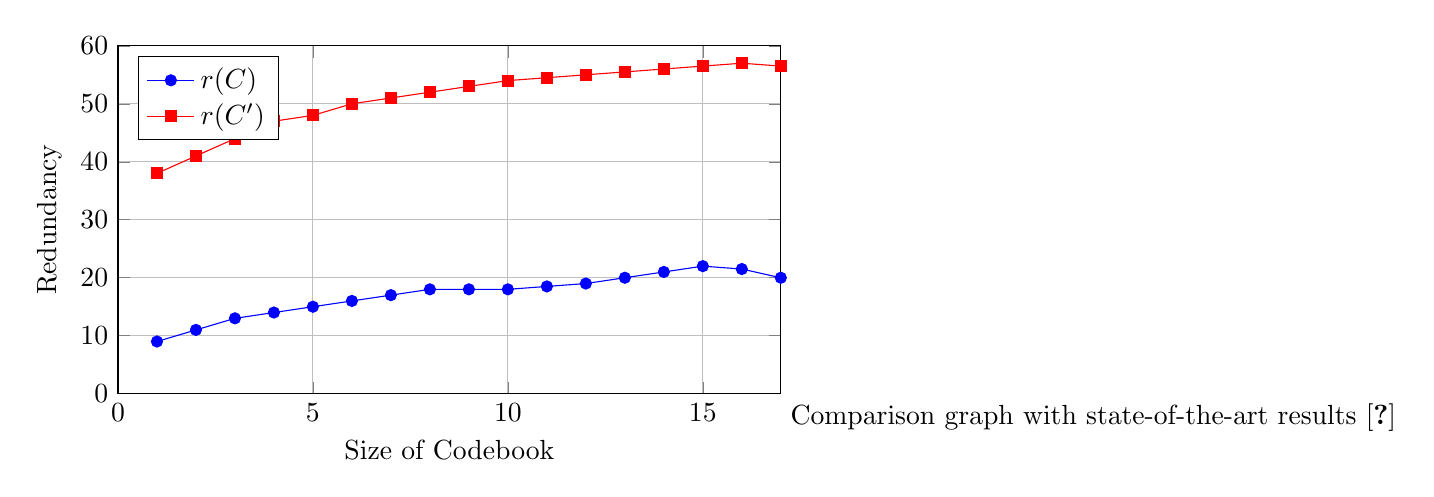
\begin{tikzpicture}
  \begin{axis}[
    width=10cm,
    height=6cm,
    xlabel={Size of Codebook},
    ylabel={Redundancy},
    xmin=0, xmax=17,
    ymin=0, ymax=60,
    xtick={0,5,...,17},
    ytick={0,10,...,60},
    legend pos=north west,
    grid=major,
    legend cell align={left},
  ]
    \addplot[
      color=blue,
      mark=*,
      ] coordinates {
        (1,9)(2,11)(3,13)(4,14)(5,15)(6,16)(7,17)(8,18)(9,18)(10,18)(11,18.5)(12,19)(13,20)(14,21)(15,22)(16,21.5)(17,20)
      };
      \label{plot1}
    \addlegendentry{$r(C)$}

    \addplot[
      color=red,
      mark=square*,
      ] coordinates {
        (1,38)(2,41)(3,44)(4,47)(5,48)(6,50)(7,51)(8,52)(9,53)(10,54)(11,54.5)(12,55)(13,55.5)(14,56)(15,56.5)(16,57)(17,56.5)
      };
      \label{plot2}
    \addlegendentry{$r(C')$}
  \end{axis}

  \node[below right] at (current axis.south east) {
    Comparison graph with state-of-the-art results \cite{Smagloy_Welter_Wachter-Zeh_Yaakobi_2020}
  };
\end{tikzpicture}

\end{document}